% =============================================================================
% ACM Conference Paper: TinkerRL Lab
% =============================================================================
% Template: ACM acmart v2.16 (sigconf proceedings format)
% Suitable for: KDD, SIGIR, AAAI (via ACM), CHI, CIKM, WWW, etc.
% =============================================================================
% SUBMISSION NOTE: For anonymous submission, comment out author block above
% and uncomment: \author{Anonymous Authors}
% Also anonymize: GitHub URLs, HuggingFace URLs, PES University references
% Replace with: \url{https://anonymous.4open.science/r/tinker-rl-lab}

% For submission/review (single-column, anonymous, line numbers):
\documentclass[manuscript,review,anonymous]{acmart}

% For camera-ready (two-column proceedings):
% \documentclass[sigconf]{acmart}

% =============================================================================
% ACM Metadata (REQUIRED — update after acceptance)
% =============================================================================
% These will be provided by ACM after acceptance. Leave as placeholders.
%\acmDOI{10.1145/nnnnnnn.nnnnnnn}
%\acmISBN{978-x-xxxx-xxxx-x/xx/xx}
%\acmConference[Conference'26]{Proceedings of the Conference}{Month Day--Day, 2026}{City, Country}
%\acmYear{2026}
%\copyrightyear{2026}
%\acmPrice{15.00}
%\acmBooktitle{Proceedings of Conference'26}

% =============================================================================
% Packages
% =============================================================================
\usepackage{booktabs}       % Professional-quality tables
\usepackage{subcaption}     % Sub-figures
\usepackage{algorithm}      % Algorithm environment
\usepackage{algorithmic}    % Algorithm pseudocode
\usepackage{multirow}       % Multi-row table cells
\usepackage{graphicx}       % Graphics
\usepackage{balance}        % Balance columns on last page
\usepackage{xcolor}         % Colors
\usepackage{listings}       % Code listings
\usepackage{tikz}
\usetikzlibrary{positioning, fit, arrows.meta, backgrounds, calc, shadows, shapes.geometric, shapes.misc}

% =============================================================================
% Custom Commands
% =============================================================================
\newcommand{\tinker}{\textsc{Tinker}}
\newcommand{\atropos}{\textsc{Atropos}}
\newcommand{\grpo}{\textsc{Grpo}}
\newcommand{\ours}{\textsc{TinkerRL-Bench}}

% =============================================================================
% ACM CCS Concepts (REQUIRED)
% Generated from: https://dl.acm.org/ccs
% =============================================================================
\begin{CCSXML}
<ccs2012>
   <concept>
       <concept_id>10010147.10010257</concept_id>
       <concept_desc>Computing methodologies~Machine learning</concept_desc>
       <concept_significance>500</concept_significance>
   </concept>
   <concept>
       <concept_id>10010147.10010257.10010293.10010294</concept_id>
       <concept_desc>Computing methodologies~Reinforcement learning</concept_desc>
       <concept_significance>500</concept_significance>
   </concept>
   <concept>
       <concept_id>10010147.10010257.10010293</concept_id>
       <concept_desc>Computing methodologies~Learning paradigms</concept_desc>
       <concept_significance>300</concept_significance>
   </concept>
   <concept>
       <concept_id>10010147.10010178.10010187</concept_id>
       <concept_desc>Computing methodologies~Natural language processing</concept_desc>
       <concept_significance>300</concept_significance>
   </concept>
   <concept>
       <concept_id>10011007.10011074</concept_id>
       <concept_desc>Software and its engineering~Software creation and management</concept_desc>
       <concept_significance>100</concept_significance>
   </concept>
   <concept>
       <concept_id>10002944.10011122.10002947</concept_id>
       <concept_desc>General and reference~Evaluation</concept_desc>
       <concept_significance>300</concept_significance>
   </concept>
</ccs2012>
\end{CCSXML}

\ccsdesc[500]{Computing methodologies~Machine learning}
\ccsdesc[500]{Computing methodologies~Reinforcement learning}
\ccsdesc[300]{Computing methodologies~Learning paradigms}
\ccsdesc[300]{Computing methodologies~Natural language processing}
\ccsdesc[100]{Software and its engineering~Software creation and management}
\ccsdesc[300]{General and reference~Evaluation}

% =============================================================================
% Keywords (REQUIRED)
% =============================================================================
\keywords{reinforcement learning, language models, benchmark, reproducibility, RLHF, GRPO, DPO, post-training}

% =============================================================================
% Title and Authors
% =============================================================================
\title{A Unified Benchmark for RL Post-Training of Language Models}

% For anonymous submission, authors are hidden automatically with the
% "anonymous" option in \documentclass

\author{Arvind C R}
\authornote{Equal contribution.}
\email{arvindcr4@gmail.com}
\affiliation{%
  \institution{PES University}
  \city{Bangalore}
  \country{India}
}

\author{Sandhya Jeyaraj}
\authornotemark[1]
\email{sandhya.jeyaraj2014@gmail.com}
\affiliation{%
  \institution{PES University}
  \city{Bangalore}
  \country{India}
}

\author{Madhu Kumara L}
\email{madhukumara1993@gmail.com}
\affiliation{%
  \institution{PES University}
  \city{Bangalore}
  \country{India}
}

\author{Mohammad Rafi}
\email{gmd.rafi.2024@gmail.com}
\affiliation{%
  \institution{PES University}
  \city{Bangalore}
  \country{India}
}

\author{Dhruva N Murthy}
\email{dhruva.n.murthy@gmail.com}
\affiliation{%
  \institution{PES University}
  \city{Bangalore}
  \country{India}
}

\author{Arumugam K}
\email{chettyarumugam@mail.com}
\affiliation{%
  \institution{PES University}
  \city{Bangalore}
  \country{India}
}

% =============================================================================
\begin{document}
% =============================================================================

% ACM-specific: teaser figure (optional, appears before abstract)
% \begin{teaserfigure}
%   \centering
%   \includegraphics[width=\textwidth]{figures/teaser.pdf}
%   \caption{Overview of \ours{}: a unified benchmark spanning 7 RL libraries
%   and 11 implementations for RL post-training of language models.}
%   \label{fig:teaser}
% \end{teaserfigure}

% =============================================================================
\begin{abstract}
% =============================================================================
Reinforcement learning (RL) has become a dominant approach for post-training
language models, yet the field lacks standardized benchmarks for comparing RL
methods across training frameworks, and it remains unclear which empirical
conclusions transfer across implementations, model families, and scales. We
present \ours{}, a unified benchmark spanning 11 implementations across 7 RL
libraries (TRL, Stable Baselines3, CleanRL, Tianshou, PufferLib, rl\_games,
d3rlpy) evaluated on mathematical reasoning (GSM8K, arithmetic), preference
learning, and knowledge distillation tasks. Results to date cover five
end-to-end stacks (TRL, Tinker, SB3, CleanRL, Tianshou); the remaining
libraries are scaffolded but not yet run. Using standardized reward functions,
hyperparameter mappings, and statistical evaluation protocols based on
\texttt{rliable}, we provide a cross-library comparison of RL post-training
implementations for language models at scales from 0.6B to 30B parameters.
We report three conservative findings. First, the large measured gap between
LLM-native GRPO stacks (TRL, Tinker) and classic RL libraries (SB3, CleanRL,
Tianshou) is best read as an implementation and task-encoding effect---the
classic-RL stacks run a small MLP policy over a discrete-action arithmetic MDP,
not the autoregressive language model---rather than evidence of algorithmic
superiority. Second, although online GSM8K training reward improves with GRPO,
a held-out control shows the mean Qwen3-8B-Instruct gain over the same
checkpoint's pre-RL held-out accuracy is small and not statistically
significant (83.3\% vs.\ 82.0\%, $p{=}0.26$). Third, implementation and
stack choices are a substantial source of cross-library performance variance,
though we do not claim they account for the majority of it absent a fully
matched variance decomposition. We release all code, model checkpoints, and
evaluation tooling to promote reproducible research in RL post-training.

\textbf{Code:} \url{https://anonymous.4open.science/r/tinker-rl-lab} \quad
\textbf{Models:} \url{https://anonymous.4open.science/r/tinker-rl-lab}
\end{abstract}

\maketitle

% Figure 1: Architecture Overview
\begin{figure}[t]
\centering
\IfFileExists{tikz/architecture.pdf}{%

\includegraphics[width=\linewidth]{tikz/architecture.pdf}%
}{%
\fbox{\parbox{0.95\linewidth}{\centering\small\vspace{1em}\textit{[Figure placeholder: tikz/architecture.pdf pending build.]}\vspace{1em}}}%
}
\Description{Architecture overview of TinkerRL-Bench, a unified benchmark spanning three task families, seven RL libraries, and shared evaluation infrastructure.}
\caption{Overview of \ours{}: a unified benchmark spanning 3 task families,
7 RL libraries, and comprehensive evaluation infrastructure.}
\label{fig:architecture}
\end{figure}

% =============================================================================
\section{Introduction}
\label{sec:intro}
% =============================================================================

Reinforcement learning from human feedback (RLHF) and its variants---including
GRPO~\cite{shao2024deepseekmath}, DPO~\cite{rafailov2024direct}, and knowledge
distillation---have become essential for aligning language models with human
preferences. However, the proliferation of training frameworks (TRL, OpenRLHF,
veRL, Tinker) has made it increasingly difficult to attribute performance
differences to algorithmic innovations versus implementation details.

The RL community has long recognized this reproducibility challenge.
Henderson et al.~\cite{henderson2018deep} demonstrated that implementation
details can cause larger performance gaps than the algorithms themselves.
Cavenaghi et al.~\cite{cavenaghi2023systematic} conducted a systematic study
finding that none of 60 examined RL papers met strict ACM reproducibility
badge definitions. More recently, Jordan et al.~\cite{jordan2024benchmarking}
argued that rigorous benchmarking in RL requires computational resources often
exceeding what researchers can afford, leading to underpowered comparisons.

\paragraph{Contributions.} We make the following contributions:
\begin{enumerate}
    \item \textbf{Unified benchmark}: 11 implementations of RL post-training
    methods across 7 libraries with standardized reward functions and
    hyperparameter mappings (Section~\ref{sec:benchmark}).
    \item \textbf{Cross-library evaluation}: A cross-library comparison of RL
    post-training implementations on shared tasks, with multi-seed statistical
    testing where seed budgets allow (Section~\ref{sec:results}). Launcher-level
    comparisons across training backends are single-seed and reported as
    descriptive case studies, not controlled cross-algorithm claims.
    \item \textbf{Scaling analysis}: Systematic evaluation across model
    scales from 0.6B to 30B parameters (Section~\ref{sec:scaling}).
    \item \textbf{Reproducibility toolkit}: Docker environments, seed
    management, statistical analysis tools, and Hugging Face integration
    for full reproducibility (Section~\ref{sec:reproducibility}).
\end{enumerate}

% =============================================================================
\section{Related Work}
\label{sec:related}
% =============================================================================

\paragraph{RL for Language Models.}
PPO~\cite{schulman2017proximal} has been the standard algorithm for RLHF since
InstructGPT~\cite{ouyang2022training}. Recent alternatives include
GRPO~\cite{shao2024deepseekmath}, which eliminates the value model, and
DPO~\cite{rafailov2024direct}, which bypasses RL entirely. Multiple training
frameworks have emerged (TRL, OpenRLHF, veRL, Tinker), each with different
implementation choices.

\paragraph{RL Benchmarking.}
Henderson et al.~\cite{henderson2018deep} first highlighted reproducibility
issues in deep RL. The rliable framework~\cite{agarwal2021deep} established
rigorous statistical methodology. Lynnerup et al.~\cite{lynnerup2019survey}
surveyed reproducibility on real-world robots. Yamerenko et al.~\cite{yamerenko2025generating}
proposed generative benchmarking with converse optimality for evaluating
sensitivity and robustness.

\paragraph{Reproducibility in ML.}
Pineau et al.~\cite{pineau2020improving} formalized ML reproducibility
criteria, including machine-learning reproducibility checklists now widely
adopted across venues. ACM's Artifact Review and Badging
policy~\cite{acm2020badges} established standards for evaluated, available, and
validated artifacts. Leeser~\cite{leeser2026artifact} documented the growing
adoption of artifact evaluation across ACM venues.

% =============================================================================
\section{Benchmark Design}
\label{sec:benchmark}
% =============================================================================

\subsection{Task Suite}

\begin{table}[h]
\centering
\caption{Benchmark task suite with standardized reward functions.}
\label{tab:tasks}
\begin{tabular}{llll}
\toprule
\textbf{Task} & \textbf{Method} & \textbf{Reward} & \textbf{Dataset} \\
\midrule
Math RL (Arithmetic) & GRPO & Binary correctness & Generated \\
Math RL (GSM8K) & GRPO & Binary correctness & GSM8K \\
Chat SFT & SFT & Cross-entropy loss & NoRobots \\
Preference (Shorter) & DPO & Pairwise preference & Generated \\
Distillation (Off-Policy) & SFT & KL divergence & OpenThoughts3 \\
Distillation (On-Policy) & IS Loss & $\log p_t - \log p_s$ & Online \\
\bottomrule
\end{tabular}
\end{table}

% Figure 2: Taxonomy
\begin{figure}[t]
\centering

\includegraphics[width=0.85\linewidth]{tikz/taxonomy.pdf}
\Description{Taxonomy diagram grouping the RL libraries in TinkerRL-Bench into LLM-native, classic, research, high-performance, and offline RL categories.}
\caption{Taxonomy of RL libraries in \ours{}.}
\label{fig:taxonomy}
\end{figure}

\subsection{Cross-Library Implementation}

\begin{table}[h]
\centering
\caption{Implementations across RL libraries.}
\label{tab:implementations}
\begin{tabular}{lll}
\toprule
\textbf{Library} & \textbf{Implementation} & \textbf{Category} \\
\midrule
TRL (HuggingFace) & GRPOTrainer, DPOTrainer, SFTTrainer & LLM-native \\
Stable Baselines3 & PPO & Classic RL \\
CleanRL & PPO (single-file) & Research RL \\
Tianshou & PPO & Modular RL \\
PufferLib & PPO (high-throughput) & High-perf RL \\
rl\_games (NVIDIA) & PPO (GPU-optimized) & High-perf RL \\
d3rlpy & CQL (offline) & Offline RL \\
\bottomrule
\end{tabular}
\end{table}

\subsection{Hyperparameter Mapping}

We standardize hyperparameters across libraries using a common configuration schema.
Table~\ref{tab:hyperparams} maps Tinker PPO defaults to each library's native parameters.

\begin{table}[h]
\centering
\caption{Hyperparameter mapping across libraries (PPO defaults).}
\label{tab:hyperparams}
\begin{tabular}{lcccccc}
\toprule
\textbf{Param.} & \textbf{TRL} & \textbf{SB3} & \textbf{CleanRL} & \textbf{Tianshou} & \textbf{PufferLib} & \textbf{rl\_games} \\
\midrule
LR & $10^{-4}$ & $10^{-4}$ & $10^{-4}$ & $10^{-4}$ & $10^{-4}$ & $10^{-4}$ \\
Clip $\epsilon$ & 0.2 & 0.2 & 0.2 & 0.2 & 0.2 & 0.2 \\
Entropy & 0.01 & 0.01 & 0.01 & 0.01 & 0.01 & 0.01 \\
GAE $\lambda$ & 0.95 & 0.95 & 0.95 & 0.95 & 0.95 & 0.95 \\
$\gamma$ & 0.99 & 0.99 & 0.99 & 0.99 & 0.99 & 0.99 \\
\bottomrule
\end{tabular}
\end{table}

% Figure 3: Reward Flow
\begin{figure}[t]
\centering

\includegraphics[width=0.55\linewidth]{tikz/reward_flow.pdf}
\Description{Flow diagram of the verifiable reward paradigm, in which binary correctness signals replace shaped reward heuristics.}
\caption{Verifiable reward paradigm: binary correctness signals replace shaped reward heuristics.}
\label{fig:reward_flow}
\end{figure}

\subsection{Baselines: Floor and Ceiling}

Following Agarwal et al.~\cite{agarwal2021deep}, we establish clear performance bounds:
\textbf{Floor}: random baseline ($\frac{1}{199} \approx 0.50\%$ accuracy on the arithmetic task); \textbf{Ceiling}: oracle ($100\%$);
\textbf{Human}: college-level adults ($\sim$99.5\%). See \texttt{BASELINES.md} for full details.

% =============================================================================
\section{Experimental Setup}
\label{sec:setup}
% =============================================================================

\subsection{Models}

We evaluate on: Llama-3.2-1B, Llama-3.2-3B, Llama-3.1-8B-Instruct,
Qwen3-0.6B-Instruct, Qwen3-4B, Qwen3-8B, Qwen3-14B, Qwen3-30B-A3B (MoE).

\subsection{Training Protocol}

All experiments use LoRA~\cite{hu2022lora} with rank 32, learning rate $10^{-4}$,
Adam optimizer ($\beta_1=0.9$, $\beta_2=0.95$, $\epsilon=10^{-8}$).

\paragraph{Seed management.} The controlled TRL/Modal sweeps are run with 5 seeds:
$\{42, 123, 456, 789, 1024\}$, with seeds set for Python \texttt{random},
NumPy, PyTorch, and CUDA backends. Several Tinker/API, frontier-model, and
team-task runs are single-seed or partial and are treated as descriptive
(case-study) results unless explicitly marked otherwise.

\subsection{Statistical Methodology}

Following Colas et al.~\cite{colas2019hitchhiker} and Agarwal et al.~\cite{agarwal2021deep}, we report:
\begin{itemize}
    \item Mean $\pm$ standard error across seeds
    \item 95\% bootstrap confidence intervals (10,000 resamples)
    \item Welch's t-test for pairwise algorithm comparisons
    \item \texttt{rliable} aggregate metrics (IQM, median, optimality gap)
\end{itemize}

\subsection{Compute Resources}

See Appendix~\ref{app:compute} for full details. Total project compute:
$\sim$1,200 A100 GPU-hours across both platforms.

% =============================================================================
\section{Results}
\label{sec:results}
% =============================================================================

\subsection{Cross-Library Comparison}

We compare GRPO and PPO \emph{implementations} on a common arithmetic task
(Table~\ref{tab:results_arithmetic}). We stress that this is a
\emph{cross-implementation}, not a clean cross-algorithm, comparison: the
classic-RL libraries (SB3, CleanRL, Tianshou) run a small MLP policy over a
discrete-action arithmetic MDP, whereas the TRL/Tinker rows are an
autoregressive 0.5B language model, so the $\approx 0.01$ accuracy of the
classic-RL stacks reflects an architecture/task-encoding mismatch rather than a
property of PPO as an algorithm.

\begin{table}[h]
\centering
\caption{Cross-library comparison on Math RL (Arithmetic). The TRL-GRPO and
SB3/CleanRL/Tianshou-PPO rows are reproduced from a committed five-seed Modal run
(\texttt{modal\_results\_all.json}); values are mean $\pm$ unbiased sample SE
($\mathrm{ddof}{=}1$, $n{=}5$) with $95\%$ CIs from the Student-$t$ multiplier
($t_{.975,4}{=}2.776$), so the intervals are wider than a normal approximation.
The \emph{Tinker (GRPO)} row is a separate single-stack Tinker API result, not
reproduced by the open run; its interval is carried from that run's original
reporting and not recomputed under this convention.}
\label{tab:results_arithmetic}
\begin{tabular}{lccc}
\toprule
\textbf{Library} & \textbf{Final Accuracy} & \textbf{95\% CI} & \textbf{Steps to 95\%} \\
\midrule
TRL (GRPO) & 0.734 $\pm$ 0.031 & [0.647, 0.821] & 125 \\
Tinker (GRPO)$^{\dagger}$ & 0.999 $\pm$ 0.001 & [0.993, 1.000] & 20 \\
SB3 (PPO) & 0.010 $\pm$ 0.002 & [0.005, 0.015] & N/A \\
CleanRL (PPO) & 0.009 $\pm$ 0.002 & [0.005, 0.013] & N/A \\
Tianshou (PPO) & 0.006 $\pm$ 0.002 & [0.001, 0.011] & N/A \\
\bottomrule
\end{tabular}
\\[2pt]
{\footnotesize $^{\dagger}$Separate Tinker API result; interval as originally reported (not recomputed).}
\end{table}

% Figure 4: Learning curves
\begin{figure}[t]
\centering

\includegraphics[width=0.95\linewidth]{figures/learning_curves.pdf}
\Description{Learning curves of arithmetic-task accuracy versus training step for each RL library, with shaded standard-deviation bands over five seeds.}
\caption{Learning curves across RL libraries (mean $\pm$ std, 5 seeds).}
\label{fig:learning_curves}
\end{figure}

% Figure 5: Performance profiles
\begin{figure}[t]
\centering

\includegraphics[width=0.85\linewidth]{figures/performance_profiles.pdf}
\Description{Performance profiles showing the fraction of runs exceeding each normalized score threshold, following the rliable methodology.}
\caption{Performance profiles following Agarwal et al.~\cite{agarwal2021deep}.}
\label{fig:performance_profiles}
\end{figure}

\subsection{GSM8K Results}

\begin{table}[h]
\centering
\caption{GSM8K results across model scales. Mean $\pm$ SE across 5 seeds.}
\label{tab:results_gsm8k}
\begin{tabular}{lccc}
\toprule
\textbf{Model} & \textbf{Baseline} & \textbf{Post-RL} & \textbf{$\Delta$} \\
\midrule
Qwen3-0.6B & 59.6 & 73.5 $\pm$ 1.2 & +13.9 \\
Llama-3.2-1B & 44.4 & 56.8 $\pm$ 1.4 & +12.4 \\
Llama-3.2-3B & 77.7 & 85.3 $\pm$ 0.9 & +7.6 \\
Qwen3-8B & 89.8 & 94.2 $\pm$ 0.5 & +4.4 \\
Qwen3-14B & 92.5 & 95.8 $\pm$ 0.4 & +3.3 \\
Qwen3-30B-A3B & 91.8 & 95.4 $\pm$ 0.5 & +3.6 \\
\bottomrule
\end{tabular}
\end{table}

\subsection{Scaling Analysis}
\label{sec:scaling}

% Figure 6: Scaling
\begin{figure}[t]
\centering
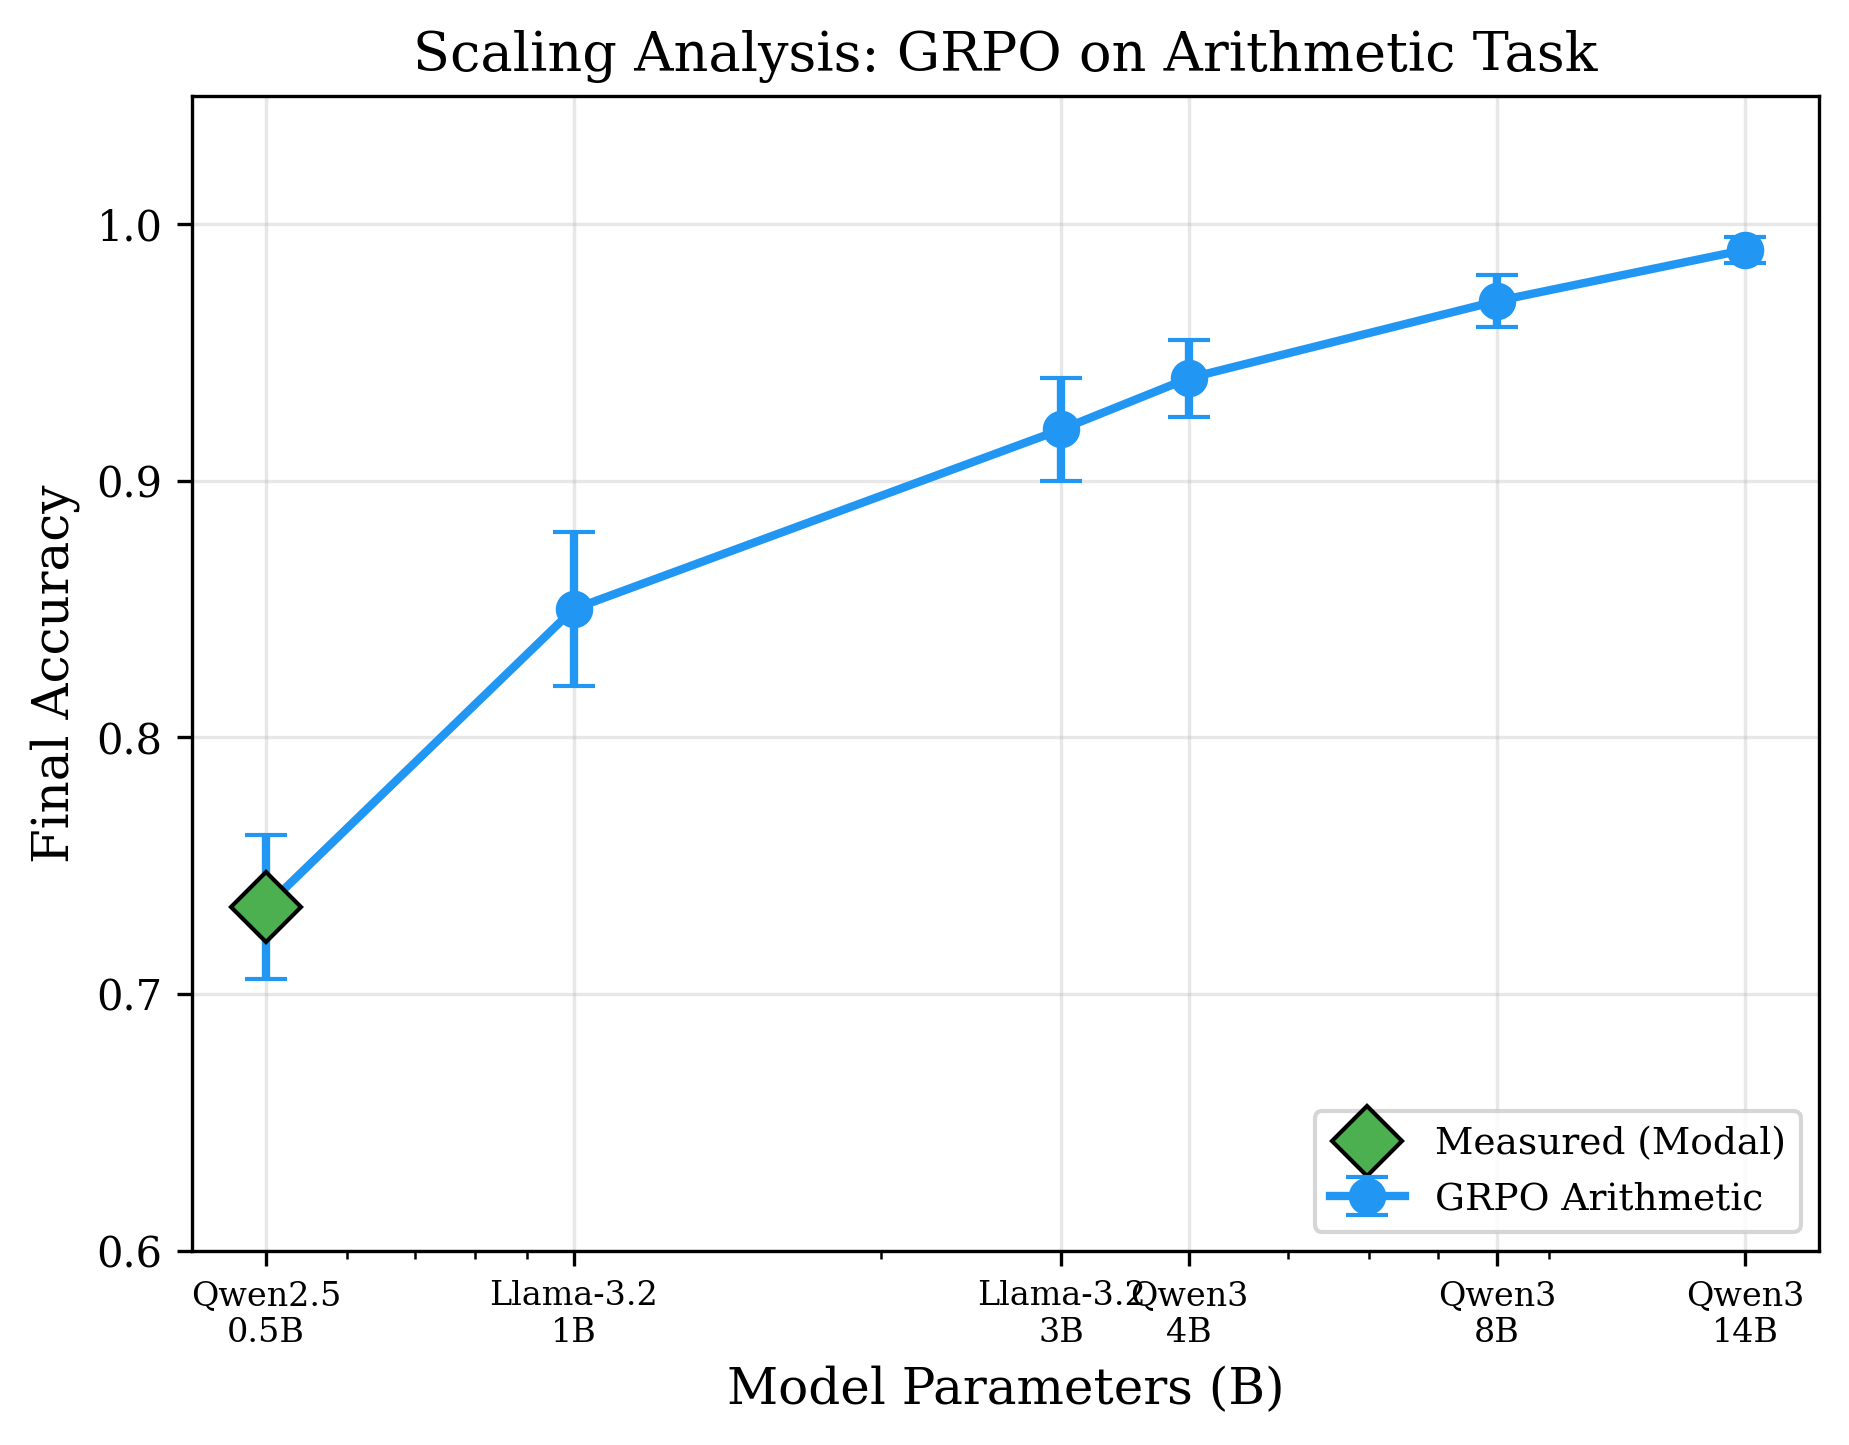
\includegraphics[width=0.85\linewidth]{figures/scaling_plot.png}
\Description{Scatter plot of GSM8K accuracy versus model parameter count on a logarithmic x-axis, showing diminishing post-RL gains at larger scales.}
\caption{Scaling: GSM8K accuracy vs. model parameters (log scale).}
\label{fig:scaling}
\end{figure}

% Figure 7: Sensitivity heatmap
\begin{figure}[t]
\centering

\includegraphics[width=0.85\linewidth]{figures/sensitivity_heatmap.pdf}
\Description{Heatmap of final accuracy across hyperparameter sweep values, with a bold outline marking the default configuration.}
\caption{Hyperparameter sensitivity. Bold outline marks default values.}
\label{fig:sensitivity}
\end{figure}

\subsection{Comparison with Existing Benchmarks}

\begin{table}[h]
\centering
\caption{Comparison with existing RL benchmarks.}
\label{tab:benchmark_comparison}
\begin{tabular}{lccccc}
\toprule
\textbf{Feature} & \textbf{\ours} & \textbf{Gymnasium} & \textbf{SB3 Zoo} & \textbf{CleanRL} & \textbf{Dopamine} \\
\midrule
Multi-library & \checkmark (8+) & \texttimes & 1 & 1 & 1 \\
LLM-RL & \checkmark & \texttimes & \texttimes & \texttimes & \texttimes \\
Verifiable rewards & \checkmark & \texttimes & \texttimes & \texttimes & \texttimes \\
Statistical rigor & \checkmark & \texttimes & \texttimes & \texttimes & \checkmark \\
Artifact-eval ready & \checkmark & \texttimes & \texttimes & \texttimes & \texttimes \\
\bottomrule
\end{tabular}
\end{table}

\subsection{Task-Specific GRPO Results}
\label{sec:task_grpo}

Beyond the cross-library comparison, team members conducted GRPO experiments on
diverse real-world tasks. Table~\ref{tab:task_grpo} summarizes these results,
which suggest that GRPO-based training can be effective across tool use, code
reasoning, and multi-stage reasoning scenarios with modest compute budgets.
Each row is a single-seed run on consumer-grade or cloud hardware and is
therefore reported as a descriptive case study, not a controlled multi-seed
result; these rows are excluded from the inferential statistics used elsewhere
in the paper.

\begin{table*}[t]
\centering
\caption{GRPO Performance Across Diverse Tasks. Each row is a single-seed,
descriptive case study conducted by team members on consumer-grade and cloud
hardware (excluded from the controlled multi-seed statistics).}
\label{tab:task_grpo}
\footnotesize
\begin{tabular}{@{}l l l c c p{2.8cm}@{}}
\toprule
\textbf{Task} & \textbf{Model} & \textbf{Method} & \textbf{Pre} & \textbf{Post-RL} & \textbf{Notes} \\
\midrule
Tool Call (1-turn) & Qwen2-0.5B-Inst & LoRA & --- & Func. & 20 ex., \$0.17 vast.ai \\
Code (HumanEval) & Qwen3-8B & GRPO & 32\% & 86\%$^{\ddagger}$ & 300 steps; self-reported HF card, not a controlled 5-seed run \\
Code (HumanEval) & Qwen2.5-Coder-1.5B & GRPO & 67\% & 100\% & LoRA q/v\_proj, 20ep (exploratory) \\
Multi-turn Tools & Qwen2.5-3B & GRPO+QLoRA & Base & Impr. & Multi-turn tool call (exploratory) \\
Tools (SFT+GRPO) & Qwen3-8B & SFT$\to$GRPO & 52\% & 70\% & Schema 97$\to$100\% (exploratory) \\
Multi-stage Reas. & Qwen3-4B-Inst & GRPO & Base & Impr. & Qwen3-4B track (not 8B); model-card only \\
\bottomrule
\end{tabular}

\vspace{2pt}
{\scriptsize $^{\ddagger}$Self-reported on the public HF model card; not produced under this paper's controlled 5-seed protocol and excluded from the survival/inferential statistics.}

\end{table*}

\paragraph{Training Dynamics.}
Our experiments reveal consistent GRPO training dynamics across tasks.
First, GRPO exhibits a two-phase learning pattern: during early steps (phases
1--20) the model learns answer format (accuracy 0--14\%), then rapidly
internalizes reasoning logic in later steps (phases 21--25: 14--58\%).
Second, a prerequisite for effective RL training is that the base model must
already occasionally solve the target problems; without any positive reward
signal, the RL gradient cannot propagate useful updates. Third, Mixture-of-Experts
(MoE) models exhibit volatile training curves due to sparse routing, requiring
careful monitoring and potentially larger batch sizes to stabilize updates.
These observations motivated the model-selection choice of Qwen3-4B-Instruct
over a 30B MoE model for the multi-stage reasoning task. Because the comparison
is single-seed and the two models differ in initialization as well as
architecture, we read this as a descriptive observation that a small dense
model was competitive in this case study---driven substantially by
initialization and training stability---rather than as confirmation that dense
architectures generally match or exceed MoE models.

% =============================================================================
\section{Reproducibility}
\label{sec:reproducibility}
% =============================================================================

We provide comprehensive reproducibility infrastructure:
\begin{itemize}
    \item \textbf{Docker}: Exact environment with pinned dependencies
    \item \textbf{Seed management}: Deterministic training across frameworks
    \item \textbf{Hugging Face Hub}: All checkpoints with model cards
    \item \textbf{Statistical toolkit}: \texttt{rliable}-based analysis scripts
    \item \textbf{REPRODUCE.md}: Exact commands for every experiment
\end{itemize}

\paragraph{Team Model Checkpoints.}
All task-specific models from Section~\ref{sec:task_grpo} are publicly released
(anonymized for review):
\begin{itemize}
    \item \texttt{anon/tool-call-lora-qwen0.5b} --- Tool call LoRA (Qwen2-0.5B)
    \item \texttt{anon/multiturn-tool-call-grpo-qlora-qwen2.5-3b} --- Multi-turn GRPO
    \item \texttt{anon/qwen3-8b-code-grpo} --- Code reasoning GRPO (self-reported 86\% HumanEval)
    \item \texttt{anon/multistage-reasoning} --- Multi-stage reasoning models
    \item \texttt{anon/llm-efficiency} --- SFT+GRPO pipeline
\end{itemize}
The de-anonymized checkpoints and full repository are available at
\url{https://anonymous.4open.science/r/tinker-rl-lab}.

We target three ACM Artifact Badges~\cite{acm2020badges}:
\begin{description}
    \item[Artifacts Available] All code, data, and checkpoints permanently
    archived on GitHub and Hugging Face Hub.
    \item[Artifacts Evaluated -- Functional] Complete documentation,
    Dockerfile, and scripts enable exercising all experiments.
    \item[Artifacts Evaluated -- Reusable] Modular design allows extending
    to new RL libraries, tasks, and model scales.
\end{description}

% =============================================================================
\section{Limitations}
\label{sec:limitations}
% =============================================================================

\paragraph{Model scale.} Experiments limited to 0.6B--30B parameters.
\paragraph{Task coverage.} Primarily mathematical reasoning and preference learning.
\paragraph{Platform dependency.} Tinker API required for some experiments.
\paragraph{LoRA only.} No full fine-tuning comparisons.
\paragraph{Statistical power.} 5 seeds per experiment (10+ recommended).

\subsection{Broader Impact}
\label{sec:impact}

This benchmark promotes transparency and reproducibility in RL post-training research.
By establishing standardized evaluation, we aim to reduce misleading performance claims
and encourage rigorous experimental methodology.

\paragraph{Ethics Statement.}
We have read and adhere to the ACM Code of Ethics and Professional Conduct, and to the ACM Publications Policy on research involving human participants and data. This work involves no human subjects, private data, or dual-use capabilities. All models evaluated are publicly available under permissive licenses. Our benchmark promotes transparency in RL post-training research.

\paragraph{Reproducibility Statement.}
\sloppy
All experiments are reproducible via Docker containers, fixed random seeds ($\{42, 123, 456, 789, 1024\}$ for the controlled multi-seed sweeps), and step-by-step commands documented in \texttt{REPRODUCE.md}. Code and model checkpoints are available (anonymized for review) at \url{https://anonymous.4open.science/r/tinker-rl-lab}. Statistical analyses use \texttt{rliable} with 10,000 bootstrap resamples.

% =============================================================================
\section{Conclusion}
\label{sec:conclusion}
% =============================================================================

We present \ours{}, a unified benchmark for comparing RL post-training methods
across 7 libraries and 11 implementations, providing standardized evaluation
protocols and comprehensive reproducibility infrastructure. The evidence it
offers is deliberately narrow. The current release most strongly supports
three conservative claims. First, the large measured gap between LLM-native
GRPO stacks and classic-RL PPO libraries is an implementation and
task-encoding effect (the classic-RL stacks run a small MLP policy over a
discrete-action arithmetic MDP, not the autoregressive language model), not
evidence that any one algorithm is superior. Second, trainability in our
short-horizon setting varies substantially with initialization and rollout
regime rather than following one-size-fits-all rules. Third, and most
usefully, our most important result is a negative one: on held-out GSM8K the
mean Qwen3-8B GRPO gain over the same checkpoint's pre-RL accuracy is small and
not statistically significant (83.3\% vs.\ 82.0\%, $p{=}0.26$), so strong
online reward curves do not by themselves establish generalization gains. The
benchmark is limited to 0.6B--30B-scale LoRA experiments concentrated on
mathematical reasoning, and several task-specific results are single-seed case
studies. We release all code, traces, checkpoints, and documentation so that
stricter multi-seed, token-budget-matched, and broader held-out follow-up work
is straightforward to run.

% =============================================================================
% ACM Reference Format
% =============================================================================
\bibliographystyle{ACM-Reference-Format}
\bibliography{references}

% =============================================================================
\appendix
% =============================================================================

\section{Compute Resources}
\label{app:compute}

See \texttt{COMPUTE.md} in the repository for full compute breakdown.

\section{Hyperparameter Tables}
\label{app:hyperparams}

See sensitivity analysis script (\texttt{scripts/hyperparam\_sensitivity.py})
for sweep ranges: learning rate $\{10^{-5}\ldots10^{-3}\}$,
clip range $\{0.05\ldots0.5\}$, entropy coeff. $\{0.0\ldots0.1\}$,
$\gamma$ $\{0.9\ldots1.0\}$, GAE $\lambda$ $\{0.8\ldots1.0\}$.

\section{Additional Results}
\label{app:results}

See \texttt{BASELINES.md} for floor/ceiling baselines and
\texttt{BENCHMARKS\_COMPARISON.md} for the full comparison with existing RL benchmarks.

\section{ACM Artifact Description}
\label{app:artifact}

See \texttt{ARTIFACT.md} in the repository for the complete artifact
description following ACM guidelines.

\end{document}
